\chapter{Evaluation}
In this chapter, the tool will be put in to test with two computational model, influenza1918 and Covasim. Influenza1918 is a relatively simple model compare to Covasim, this chapter will go through the testing process more both model, and the result produced, then some discussion about the result.
\section{Testing influenza1918}
Influenza1918 is an equation-based model originally developed to for the need to design model validation strategies, this is a model that simulate epidemiological disease-spread of the course of the 1918 Influenza epidemic within the United States.
This model has five state variables and six parameters [influenze1918 REFERENCE].\\*\\*
\subsection{Testing process for influenza1918}
First, a scenario name influenza1918 is created, 
\begin{figure}[H]
	\centering
	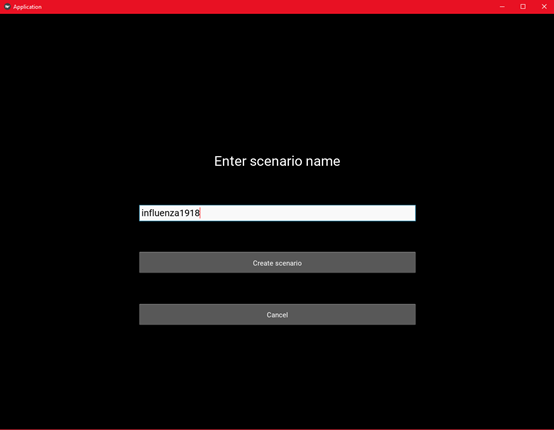
\includegraphics[width=10cm]{figures/influenzaTestProcess1.png}\\
	\caption{Creating new scenario for influenza1918.}
	\label{fig:figure19}
\end{figure}
Since influenza1918 is implemented through OpenModelica in a \textsl{influenza1918.mo} file, so to test this model, first user need to put the model file into the \textsl{\textbackslash scenarios\textbackslash influenza1918 \textbackslash model}. Next use the “Edit dot files” button to start edit the relations of the parameters.
\begin{figure}[H]
	\centering
	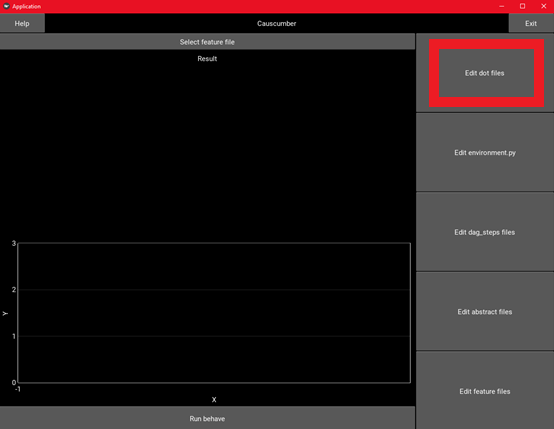
\includegraphics[width=10cm]{figures/influenzaTestProcess2.png}\\
	\caption{Select “Edit dot files” function.}
	\label{fig:figure20}
\end{figure}
A file named influenza1918\_abstract is created, there are two graph needed, first is \textsl{cluster\_inputs} with the input parameters, then \textsl{cluster\_outputs} with the output parameters. In the right panel, enter the file name influenza1918\_abstract, then select the type of graph, input the graph name and label, and the parameters for the selected cluster, click add graph to apply the change.
\begin{figure}[H]
	\centering
	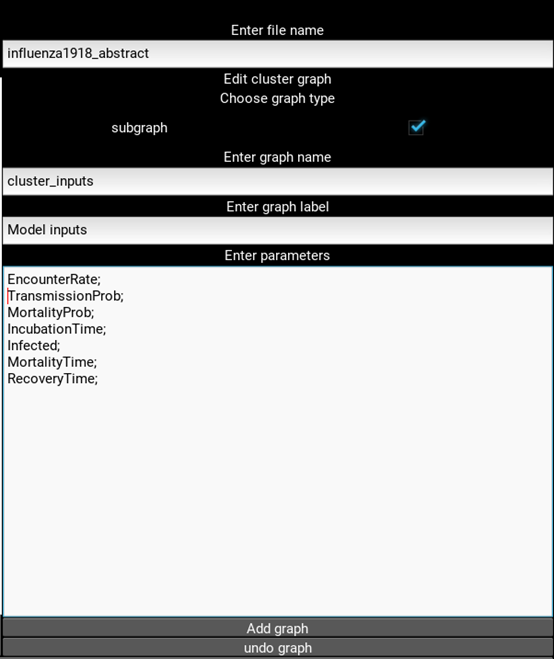
\includegraphics[width=10cm]{figures/influenzaTestProcess3.png}\\
	\caption{Edit graph for input parameters.}
	\label{fig:figure21}
\end{figure}
\begin{figure}[H]
	\centering
	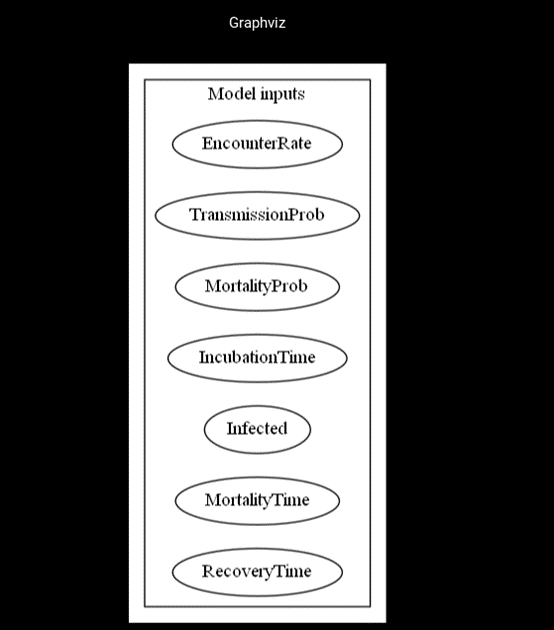
\includegraphics[width=10cm]{figures/influenzaTestProcess4.png}\\
	\caption{Graphviz for input parameters graph.}
	\label{fig:figure22}
\end{figure}
After added the graph, the left panel will then display the graph via Graphviz. Next is edit the relations between these parameters.
\begin{figure}[H]
	\centering
	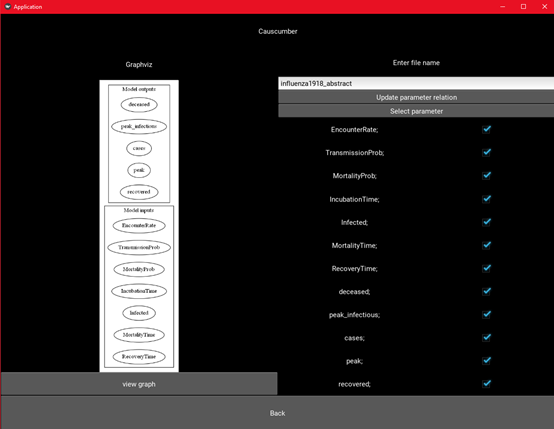
\includegraphics[width=10cm]{figures/influenzaTestProcess5.png}\\
	\caption{Edit relation for parameters.}
	\label{fig:figure23}
\end{figure}
First, select the file, then select the parameters that are going to be affected via the checkboxes, then select the parameters that are going to affect them via the drop-down menu, then the left panel will be updated.
\begin{figure}[H]
	\centering
	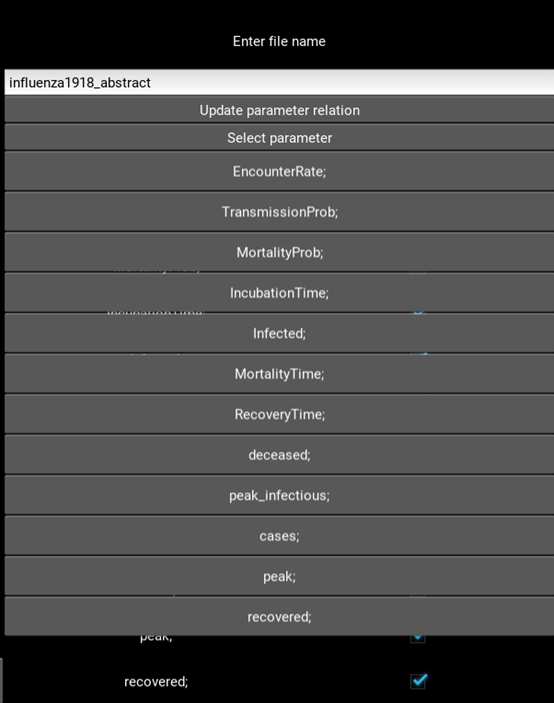
\includegraphics[width=10cm]{figures/influenzaTestProcess6.png}\\
	\caption{Drop-down menu for select parameter.}
	\label{fig:figure24}
\end{figure}
\begin{figure}[H]
	\centering
	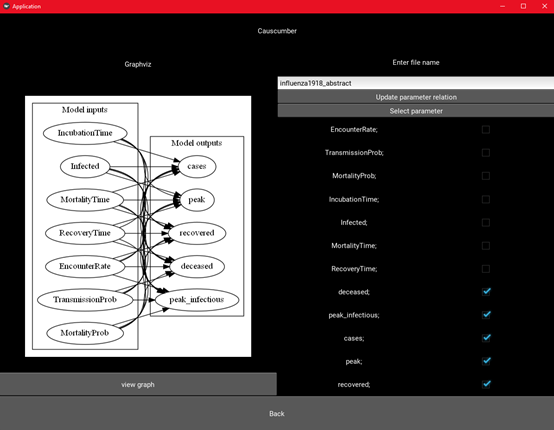
\includegraphics[width=10cm]{figures/influenzaTestProcess7.png}\\
	\caption{Relations of parameters presented in Graphviz graph.}
	\label{fig:figure25}
\end{figure}
After finishing editing the relationship, click back to return to the main menu.
Next user will need to edit the three background files, 
\begin{figure}[H]
	\centering
	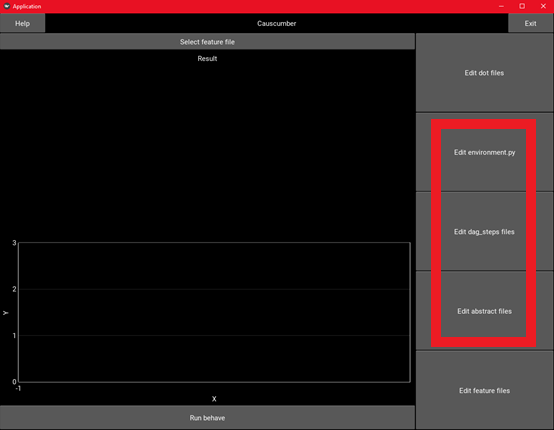
\includegraphics[width=10cm]{figures/influenzaTestProcess8.png}\\
	\caption{Edit background files for testing influenza1918.}
	\label{fig:figure26}
\end{figure}
In environment.py, edit the run\_influenza1918 function to execute the influenza1918 model. Then for dag\_steps.py, define metavariables in the background, a metavariable called “m” needs a function “populate\_m” define. Last is for abstract.py file, apply custom constrain to the parameters of the tested model. \\*\\*
Finally is the \textsl{.feature} file, use “Edit feature files” to create a feature file. 
\begin{figure}[H]
	\centering
	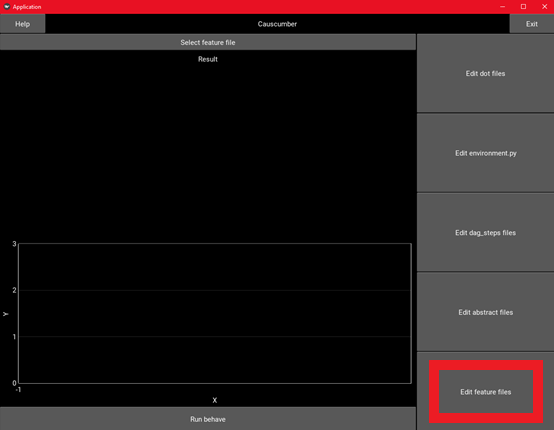
\includegraphics[width=10cm]{figures/influenzaTestProcess9.png}\\
	\caption{Edit background files for testing influenza1918.}
	\label{fig:figure27}
\end{figure}
Starting from the top user will need to define the feature file’s name, its parameters and its value/distribution and type,
\begin{figure}[H]
	\centering
	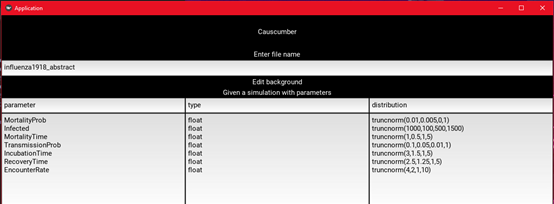
\includegraphics[width=10cm]{figures/influenzaTestProcess10.png}\\
	\caption{Edit initial parameters name, type and value/distribution in influenza1918.}
	\label{fig:figure28}
\end{figure}
Next step is to define what parameter to record and when to record, since influenza1918 doesn’t require any meta variable, that part will be left empty.
\begin{figure}[H]
	\centering
	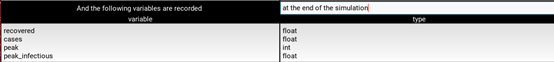
\includegraphics[width=10cm]{figures/influenzaTestProcess11.png}\\
	\caption{Edit recorded parameters name and type in influenza1918.}
	\label{fig:figure29}
\end{figure}
Next is to define the edges for the parameters, this process is same as edit dot file step. Since scenario outline is required in this case, next part will also be skip. Last is scenario, in the right panel, edit the change and expected outcome. 
\begin{figure}[H]
	\centering
	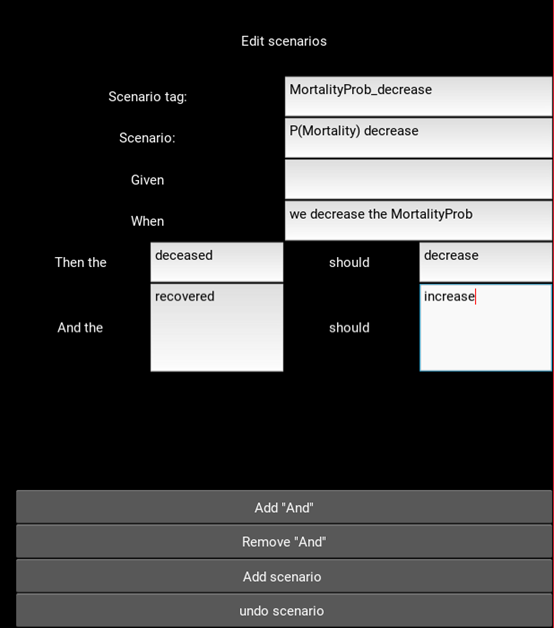
\includegraphics[width=10cm]{figures/influenzaTestProcess12.png}\\
	\caption{Edit scenario for influenza1918.}
	\label{fig:figure30}
\end{figure}
Upon finish edit all the scenario, user can then return to main menu and then select the feature file
\begin{figure}[H]
	\centering
	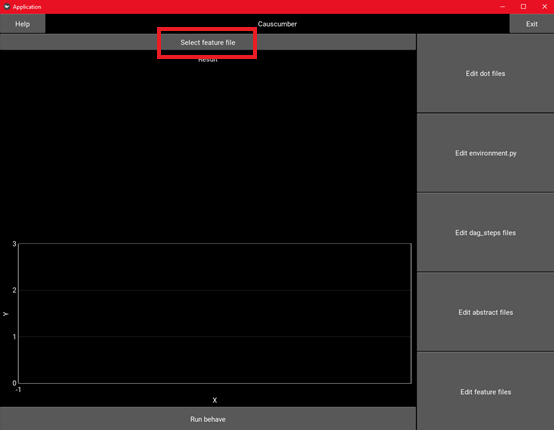
\includegraphics[width=10cm]{figures/influenzaTestProcess13.png}\\
	\caption{Select “Select feature files” function.}
	\label{fig:figure31}
\end{figure}
\begin{figure}[H]
	\centering
	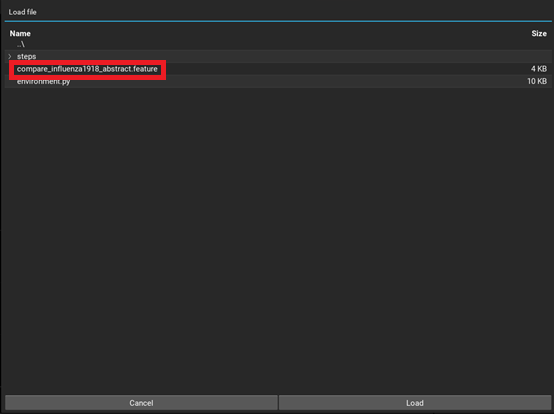
\includegraphics[width=10cm]{figures/influenzaTestProcess14.png}\\
	\caption{Select newly created feature file.}
	\label{fig:figure32}
\end{figure}
After select feature file, user run behave to produce the result on the screen,
\begin{figure}[H]
	\centering
	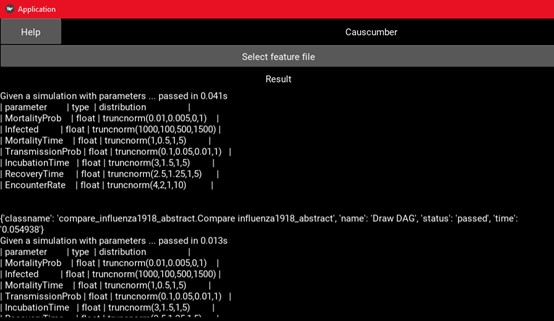
\includegraphics[width=10cm]{figures/influenzaTestProcess15.png}\\
	\caption{Result produced by Causcumber display in result section.}
	\label{fig:figure33}
\end{figure}

\subsection{Testing result for influenza1918}
In the result produced by Causcumber, in the test carryout with the assisting tool or without, all produce the same result. In the files produced by the tool, starting with \textsl{.dot} file, it is identical with manually created version with some minor difference in formats that doesn’t matter in this case. With this assist of the tool, this process also become a lot more efficient. Next are the three background files, in those files, most of the parts are already pre-define with some parts that can only be manually define by user. Last, in \textsl{.feature} file, the file generated by the tool is no difference compare to the manually created file, and by splitting the files into different sections, and edit it one by one, it become more streamline and readable from a user’s point of view. 
\subsection{Discuss result}
With the assisting tool, creating test for influenza are relatively simplify because as a user, it is not necessary to understand all the syntax for all the files. And with the auto generated files, since not all the parts require manually input, the chance of error occur has been reduced. One of the problem originally user may encounter when define edges for files such as \textsl{.dot} file and \textsl{.feature} file, is that it is difficult for user to list all the edges without any sort of visualization. With the Graphviz’s assist, this process become much clearer during the process. Unfortunately, for the three background files, part of it still require user to manually code those parts in due to the methods use by developers to code computational model maybe drastic different.

\section{Testing Covasim}
Covasim is an agent-based model pf COVID-19 dynamics and interventions, it simulate individual people as an agent, agents will be assigned different states such as infectious or recovered, agents can change to different states and in each states can provide different affects to the simulations. Agents will also be affected by the “Interventions” such as masks or physical distancing. Compare to influenza1918 models in the previous section, this model is a lot more complex with more parameters and methods. 
\subsection{Testing process for Covasim}





